\section{Analysis}
\label{sec:analysis}

\subsection{Where the Baseline Loses Accuracy}
\label{sec:gap}
On ImageNet-R, training once on all 200 classes gives $A_B=86.52$, $3.9$ points
above the baseline (per-task values in Table~\ref{tab:gap},
Appendix~\ref{app:gap}). The gap sits in the oldest classes: tasks~0 and~1
lose $9.0$ and $8.3$ points, while the newest task matches joint training. The
extra errors are cross-task: per pair of classes, the ratio of cross-task to
within-task confusions is $1.38$ for the baseline and $0.90$ for joint
training. Exact statistics do not close the gap: giving the classifier
alignment the oracle statistics of old classes adds only $+0.195$ to $\bar A$;
it lifts task~0 from $80.1$ to $87.1$, but newer tasks drop. The remaining
errors are overlaps between tasks in the learned representation.

\subsection{Every Training-Time Change Trades New for Old}
\label{sec:frontier}

\begin{figure}[t]
\centering
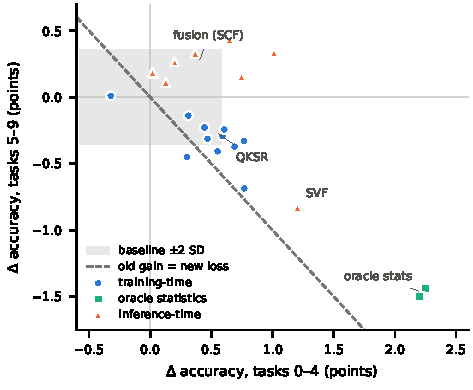
\includegraphics[width=\columnwidth]{figures/frontier.pdf}
\caption{Change of final accuracy on the old (tasks 0--4) and new (tasks 5--9)
halves against the baseline, ImageNet-R seed 1993, for every stored run and
head. Grey box: $\pm2$ SD of the five stored baseline runs of this seed. Points on the dashed line
gain on old tasks exactly what they lose on new ones.}
\label{fig:frontier}
\end{figure}

Figure~\ref{fig:frontier} places every stored run and head on ImageNet-R seed
1993 by the change of its old- and new-half accuracy (61 stored runs over all
datasets enter the analysis). This analysis is post hoc; its reading criteria
were written before running the script.
\begin{itemize}
  \item \emph{Training-time interventions trade.} None of the 11 runs that
    change the adapter (6 QKSR, 3 Holevo, 2 POVM) raises both halves. All 5
    that move the old half by more than two standard deviations keep final
    accuracy within two standard deviations; they lose a median $0.49$ points
    on new tasks per point gained on old ones, so $\bar A$ stays flat.
  \item \emph{Oracle statistics move furthest along the same line}: old
    $+2.2$, new $-1.5$.
  \item \emph{Only fusion raises both halves}: 28 of 37 inference-time points
    over all datasets. A snapshot-view head, which fuses the linear
    head with ridge scores on the features of the frozen task-0 network, is
    also inference-time but trades like the training-time changes, so our pre-registered criterion, which
    grouped the two, was not met.
\end{itemize}
The quantum regularisers therefore did not fail for quantum reasons: within
a shared adapter, separating old from new classes moves accuracy along a
trade-off curve rather than above it.

\subsection{Why the Separation Kernel Fails}
\label{sec:qksr-analysis}

\begin{table}[t]
\centering
\small
\setlength{\tabcolsep}{3pt}
\begin{tabular}{lr}
\toprule
Probe quantity (median over tasks 1--9) & Value \\
\midrule
Class AUC, cosine on $\mathbf z$ (768-d) & 0.95 \\
Class AUC, Euclidean on $\mathbf z$ & 0.85 \\
Class AUC, RBF on the 8 angles & 0.72 \\
Class AUC, PQK distance & 0.59 \\
\quad PQK at task 0 / task 9 & 0.76 / 0.57 \\
Angles with $|\theta|>0.9\pi$ & 43\% \\
Between-class scatter in projector span & $3.9\times$ random \\
Kernel, top-5 nearest old means / all & 0.85 / 0.56 \\
\midrule
cos(classification, separation gradient) & $-0.002$ \\
$\|$separation$\|$ / $\|$classification$\|$ gradient & 0.24 \\
cos(classification, alignment gradient) & $-0.14$ \\
\bottomrule
\end{tabular}
\caption{Read-only probe of the QKSR run (ImageNet-R, seed 1993). AUC: probability
that a different-class pair is farther apart than a same-class pair.}
\label{tab:probe}
\end{table}

Table~\ref{tab:probe} locates the weaknesses of the separation kernel. The
768-dimensional features separate classes well, but the 8-angle projection
keeps little of it, and the circuit loses more (AUC $0.85\to0.72\to0.59$).
Because the projection is frozen after task~0, it degrades from task to task
(Figure~\ref{fig:probe-auc}, Appendix~\ref{app:figures}),
and 43\% of the angles saturate the $\tanh$. The separation gradient is nearly
orthogonal to the classification gradient and a quarter of its size, so it
moves the adapter in directions irrelevant to classification; there is no
gradient conflict for methods such as auxiliary-gradient
projection~\citep{dery2021attittud} to remove, and tuned loss weights
generally match such methods anyway~\citep{xin2022mtl,kurin2022unitary}. The repair fixes the measured
weaknesses: the kernel used in training is no longer concentrated (mean
$0.06$--$0.11$ instead of $0.55$), yet accuracy drops. One reading, which we
have not tested, is that QKSR's small benefit on old tasks comes from a diffuse
push away from all old classes, which a sharper kernel concentrates on a few
near pairs. Unexpectedly, the alignment gradient opposes the classification
gradient at every probed step, in the baseline as well ($-0.15$); it is a
candidate source of the trade-off of Section~\ref{sec:frontier}.

\subsection{Error Analysis of the Measurement}
\label{sec:errors}
In the base task, where there is no drift, the PGM matches the linear head on
ImageNet-R ($-0.31$, $[-0.77,+0.15]$) and beats ridge on the same statistics
($+0.68$, $[+0.44,+0.92]$). As tasks accumulate, its deficit to the linear head
grows linearly to $-2.79$; the extra errors are old images assigned to newer
tasks ($11.5\%$ of the test set against $9.9\%$ for the linear head).
Transporting the states with a fitted channel does not change this, and oracle
states lift task~0 by $2.8$--$6.5$ points but $A_B$ by only $+0.64$. The
hierarchical measurement removes about two thirds of the deficit ($+0.33$,
$[+0.02,+0.64]$ over the flat PGM).

Stand-alone, every generative score is worse than the linear head, but they
err on different images. On ImageNet-R the PGM and the linear head disagree on
$14\%$ of the test images: the linear head is right on $5.8\%$ of them, the PGM
on $3.2\%$, and neither on $5.4\%$. Calibration is what lets fusion use this:
an uncalibrated sum follows the linear head on $87\%$ of the disagreements,
because Born probabilities are much flatter than a softmax at scale $s$, and
gains only $+0.25$ (ImageNet-R) and $+0.44$ (ImageNet-A).
\todo{Qualitative examples: test images on which the linear head and the
fused head disagree (images are not stored with the logs; recover them from
the fixed ImageNet-R split by test index).}
